\documentclass[10pt,a4paper]{article}
\usepackage[utf8]{inputenc}

\usepackage{amsmath}
\usepackage{amsfonts}
\usepackage{amssymb}
\usepackage{graphicx}
\usepackage{listings}

\lstset{numbers=left,
	title=\lstname,
	numberstyle=\tiny, 
	breaklines=true,
	tabsize=4,
	language=Python,
	morekeywords={with,super,as},,
	frame=single,
	basicstyle=\footnotesize\tt,
	commentstyle=\color{comment},
	keywordstyle=\color{keyword},
	stringstyle=\color{string},
	backgroundcolor=\color{white},
	showstringspaces=false,
	numbers=left,
	numbersep=5pt,
	literate=
		{æ}{{\ae}}1
		{å}{{\aa}}1
		{ø}{{\o}}1
		{Æ}{{\AE}}1
		{Å}{{\AA}}1
		{Ø}{{\O}}1
	}

\usepackage{bm}
\usepackage{hyperref}
\usepackage[margin=1.25 in]{geometry}
\usepackage[usenames, dvipsnames]{color}
\usepackage{float}

\begin{document}

\begin{center}
{\LARGE\bf
FYS4150\\
Project 3, deadline October 25.
}
 
\includegraphics[scale=0.075]{uio.png}\\
Authors: Robin D. Kifle, Sander W. Losnedahl and Vemund S. Thorkildsen\\
University of Oslo, Autumn 2017

\vspace{3cm}
{\LARGE\bf
Abstract
}

\end{center}

\newpage

{\LARGE\bf
Introduction
}\\

\noindent In this report we will build a model for our solar system. The emphasis will be on creating an object oriented code and calculating the orbits of the planets. The system can be described by using a series of coupled ordinary differential equations. In the first part of the report, a simplified version of the problem will be looked at. This is the hypothetical earth-sun binary situation. Another hypothetical situation will also be looked at, namely a three body system, with Earth, Jupiter and the sun. The equations are rather simple up to three planets, but as the end goal is a system of ten celestial bodies, it will become vital to object orient the code. Preservation of kinetic and potential energy will be discussed, in addition to preservation of angular momentum. The last thing that will be looked upon is the perihelion precession of Mercury. \\

\noindent Two different algorithms will be tested. The euler forward algorithm, and the velocity verlet algorithm. Both of them are numerical integration algorithms, and will be discussed later. The code can be found \href{https://github.com/VemundStenbekkThorkildsen/Assigment3}{\textcolor{blue}{here}}. \\   





{\LARGE\bf
Method
}\\

\noindent For the earth-sun binary system, a simple algorithm was made. In this example, the suns position will be fixed. This approximation is okay to make, as the earths mass only is three millionths of the suns mass. In this system there is only one force:


$$
F_G=\frac{GM_{\odot}M_{\mathrm{Earth}}}{r^2}
$$

\noindent To use the euler or velocity verlet algorithm, the acceleration must be known. Using newtons second law of motion it it is easy to derive the acceleration. 


$$F_G=M_{Earth}*a $$

$$M_{Earth}*a=\frac{GM_{\odot}M_{\mathrm{Earth}}}{r^2} \Rightarrow a=\frac{GM_{\odot}}{r^2}$$

\noindent Eulers forward method consists of three steps. Firstly the acceleration must be known, as well as initial conditions for position and velocity. As shown above, the acceleration can be calculated easily for this case, but it needs to be decomposed into x- and y-coordinates. 

$$a_x=-G\frac{M_{\odot}}{r^2}cos(\theta)=-G\frac{M_{\odot}x}{r^3}$$
$$a_y=-G\frac{M_{\odot}}{r^2}sin(\theta)=-G\frac{M_{\odot}y}{r^3}$$

\noindent Using that $x=r*cos\theta$ and $y=r*sin\theta$.  The three steps shown for x:

$$a_t=\frac{F_G}{M_{Earth}}$$

$$v_{t+\bigtriangleup t}=v_t + a_t\bigtriangleup t $$

$$x_{t+\bigtriangleup t}=x_t + v_{t+\bigtriangleup t}\bigtriangleup t$$

\noindent The same algorithm applies for y. This algorithm is simple, and only consists of $5n$ FLOPS, but this has its effects on the accuracy. The velocity verlet algorithm can be summarized in four steps. Once again, the algorithm is viable for x- and y-dimension.  



$$v_{t+\frac{1}{2}\bigtriangleup t}=v_t + \frac{1}{2}a_t\bigtriangleup t$$

$$x_{t+\bigtriangleup t}=x_t + v_{t+\frac{1}{2}\bigtriangleup t}\bigtriangleup t $$
<<<<<<< HEAD

$$a_{t+\bigtriangleup t}=a_{t+\bigtriangleup t}$$

$$v_{t+\bigtriangleup t}=v_{t+\frac{1}{2}\bigtriangleup t} + \frac{1}{2}a_{t+\bigtriangleup t}\bigtriangleup t$$

=======

$$a_{t+\bigtriangleup t}=a_{t+\bigtriangleup t}$$

$$v_{t+\bigtriangleup t}=v_{t+\frac{1}{2}\bigtriangleup t} + \frac{1}{2}a_{t+\bigtriangleup t}\bigtriangleup t$$

>>>>>>> 218c715cc637d816f1e336e4e2e4249c1ebfb8c6
\noindent The new acceleration is computed in the third line by using the updated position. The velocity verlet algorithm uses $9n$ FLOPS, hence is more time consuming than the Euler forward algorithm. The forces acting upon Earth in the three body problem is more complex. In this case, the force acting upon earth from the sun can be described in the exact same fashion. The new element is the gravitational force of Jupiter. 

$$F_{Earth-Jupiter}=G\frac{M_{earth}M_{jupiter}}{d_{Earth-Jupiter}}$$

\noindent where $d_{Earth-Jupiter}$ is the distance between the planets. The sum of forces acting on earth in this problem: 

$$\sum F = F_{Earth-Jupiter}+ F_{Earth-Sun}= M_{earth}G(\frac{M_{jupiter}}{d_{Earth-Jupiter}} + \frac{M_{\odot}}{r^2}) $$

\noindent The same relations act upon Jupiter, but then the mass of Earth is swapped for the mass of Jupiter. The acceleration in all dimensions can be found by dividing with respective masses and decomposing using the relations showed earlier in this chapter. Continuing on this path will only lead to long equations, and headache. Consider the model for the entire solar system. The forces acting upon earth will be the sum of nine gravitational forces. The forces acting upon the remaining nine celestial bodies can also be expressed as the sum of nine gravitational forces. This underlines the importance of object orientation once again.\\

\noindent This project is well suited for an object oriented code since we have planets with given properties, or members in code language, like initial position and velocity as well as mass. Many more members could be assigned to the planet and the code would still work. \\


\noindent Each planet was made as an object, passing initial values into our body class. This class takes the the initial values and turn them into member variables, making them available to all classes in the code. The solarSystem class takes these member variables and does operations on them, such as calculating energy and force for each integration step. The integration itself is encoded in the verlet class, which actually contains both the Euler forward method and the velocity Verlet method. Which method to use is up to the user. Another feature of the solarSystem class is the printing function where the position, angular momentum, perihelion angle and distance and total energy is printed to .txt files.\\


\noindent The positions and velocities are vectors which are based on the components class. The class most of all allows for vector based operations such that one can define the position and velocities in terms of their spacial components and this makes the vectors much easier to work with. Other vector operations are also possible with this class such as finding the length of vectors, the cross product of vectors and basic algebraic operations.\\

\noindent By using conservation of energy, it is possible to derive a formula for escape velocity. The initial speed will be equal to the escape velocity $v_e$. At a later state, the planet has escaped and is positioned an infinite distance away from the sun and the speed will be close to zero. We will only account for kinetic energy, $E_k$, and gravitational potential energy, $E_p$. By conservation of energy: 
$$(E_k+E_p)_i = (E_k+E_p)_{\infty}$$
$$\Rightarrow \frac{1}{2}M_{\otimes}v_e^2 + \frac{-GM_{\odot}M_{\otimes}}{r} = 0 + 0$$
$$\Rightarrow v_e = \sqrt{\frac{2GM_{\odot}}{r}} = 2\sqrt{2}\pi \frac{AU}{yr}$$
where $M_{\otimes}$ = mass of Earth, $G$ = the gravitational constant, $M_{\odot}$ = mass of Sun, and $r$ = distance between the Earth and the Sun.\\


\noindent The perihelion precession of Mercury is an important test for the general theory of relativity. The orbit of Mercury is not a perfect circle, but an ellipse. The perihelion of mercury is not at the same place for each orbit, but is slightly shifted. This slight shift is only possible to see clearly if the there are fine integration steps. To find the perihelion, one must find the point, in each orbit, that is closer to the sun than both its immediate neighboring integration points. This is only true for one point per orbit. By using finer and finer integration partition, the precision of the perihelion will get better.   






<<<<<<< HEAD
The perihelion precession of Mercury is an important test for the general theory of relativity. The orbit of Mercury is not a perfect circle, but an ellipse. The perihelion of mercury is not at the same place for each orbit, but is slightly shifted. This slight shift is only possible to see clearly if the there are fine integration steps. To find the perihelion, one must find the point, in each orbit, that is closer to the sun than both its immediate neighboring integration points. This is only true for one point per orbit. By using finer and finer integration partition, the precision of the perihelion will get better.   

\noindent This project is well suited for an object oriented code since we have planets with given properties, or members in code language, like initial position and velocity as well as mass. Many more members could be assigned to the planet and the code would still work. 
\\
Each planet was made as an object, passing initial values into our body class. This class takes the the initial values and turn them into member variables, making them available to all classes in the code. The solarSystem class takes these member variables and does operations on them, such as calculating energy and force for each integration step. The integration itself is encoded in the verlet class, which actually contains both the Euler forward method and the velocity Verlet method. Which method to use is up to the user. Another feature of the solarSystem class is the printing function where the position, angular momentum, perihelion angle and distance and total energy is printed to .txt files.
\\
The positions and velocities are vectors which are based on the components class. The class most of all allows for vector based operations such that one can define the position and velocities in terms of their spacial components and this makes the vectors much easier to work with. Other vector operations are also possible with this class such as finding the length of vectors, the cross product of vectors and basic algebraic operations.
=======
>>>>>>> 218c715cc637d816f1e336e4e2e4249c1ebfb8c6












\newpage
{\LARGE\bf
Results
}\\
\begin{figure} [H]  

\centerline{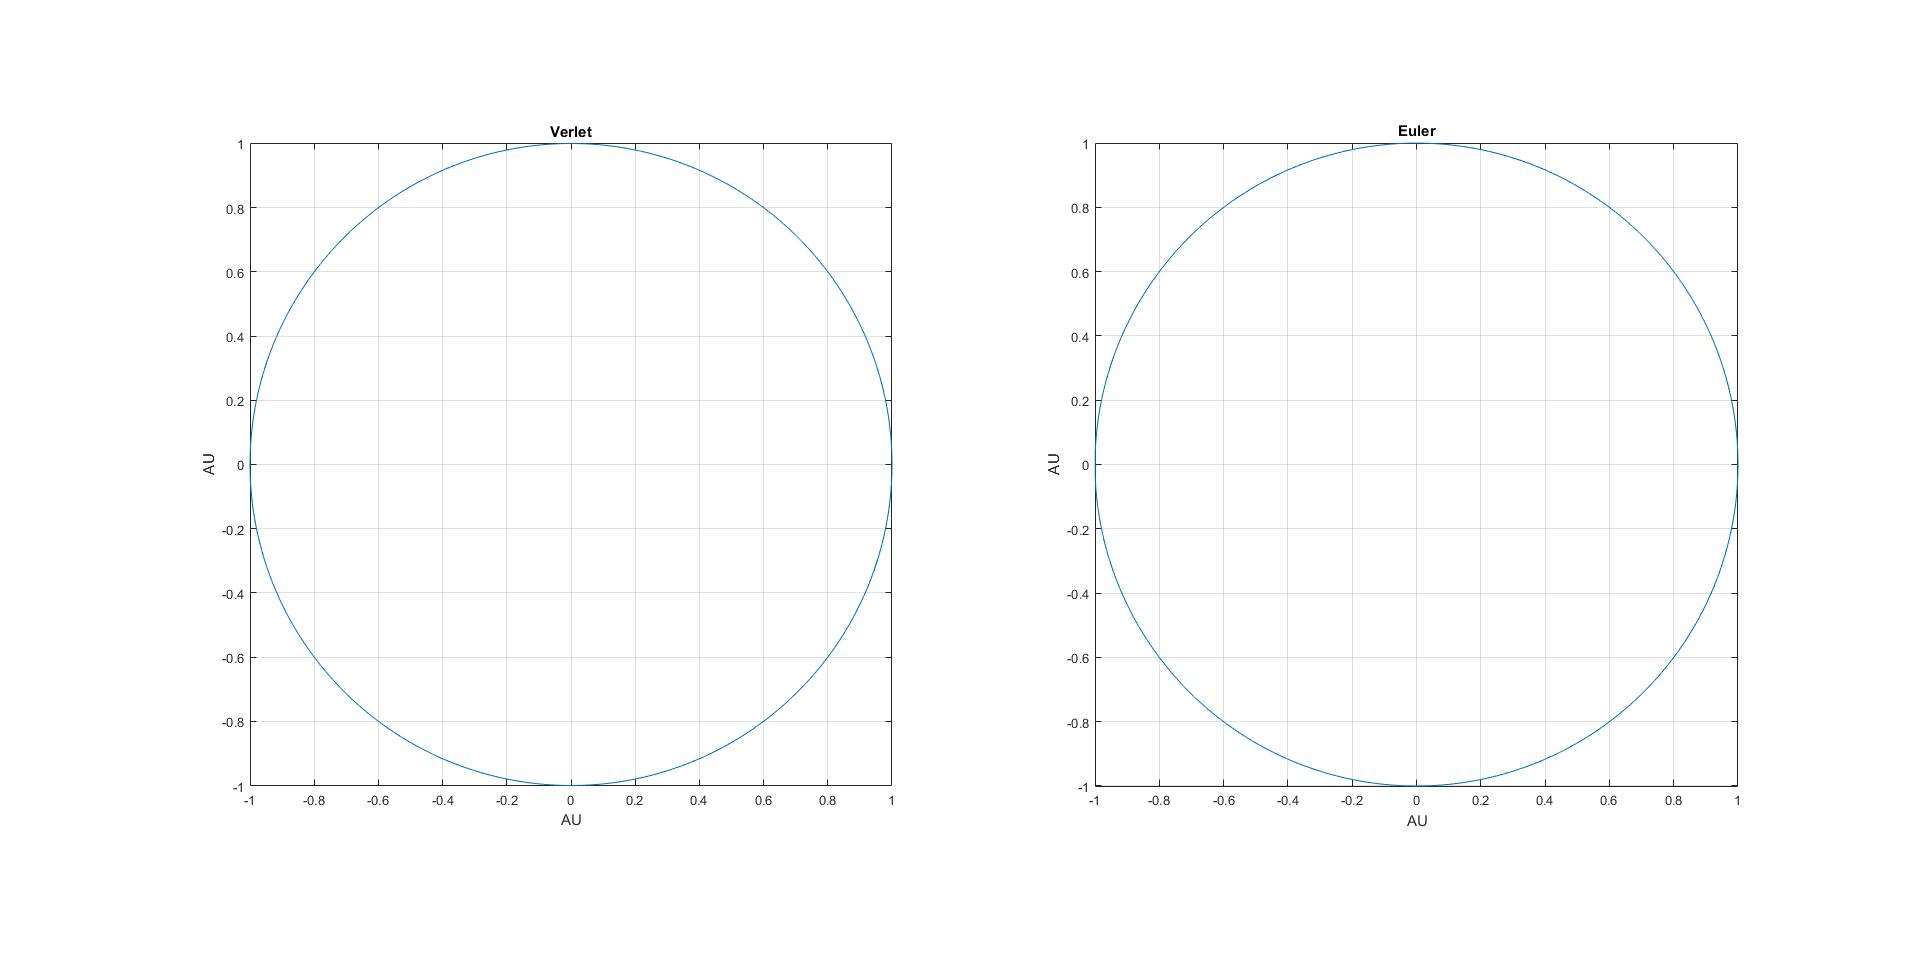
\includegraphics[scale=0.3]{FirstModel.jpg}}
\caption{The planetary orbit of Earth around the sun, with no other interfering forces. Calculated over 100 years with 10000 integration steps per year. This figure was created by using the velocity verlet algorithm}
\end{figure}

\noindent Figure 1 is showing  two models for the Earth-Sun binary system. Both are showing nearly perfect circles, but by playing around with $\bigtriangleup t$, one of the algorithms prove much more solid. As stated earlier, the euler method has fewer FLOPS, but this takes a toll on the accuracy. The velocity verlet algorithm is heavier for the computer to handle, but it gives a much better approximation for each iteration. \\ 

\begin{center}
\begin{tabular}{|c|c|c|}
\hline
  n  & Euler & velocity verlet\\
\hline
10        & 0.001s & 0.001s \\
\hline
$10^2$      & 0.001s & 0.001s \\
\hline
$10^3$      & 0.004s & 0.004s \\
\hline
$10^4$      & 0.021s & 0.018s \\
\hline
$10^5$      & 0.163s & 0.178s \\
\hline
$10^6$      & 1.614s & 1.785s \\
\hline
$10^7$      & 15.864 & 17.553 \\
\hline
$10^8$      & 159.762s & 177.366  \\
\hline
\end{tabular}\\
Table 1: Timing of the algorithms for the Earth-Sun binary system. Euler is faster than velocity Verlet for high n-values. Both algorithms show a linear increase in computing timing. 
\end{center}



\begin{figure} [H]

\centerline{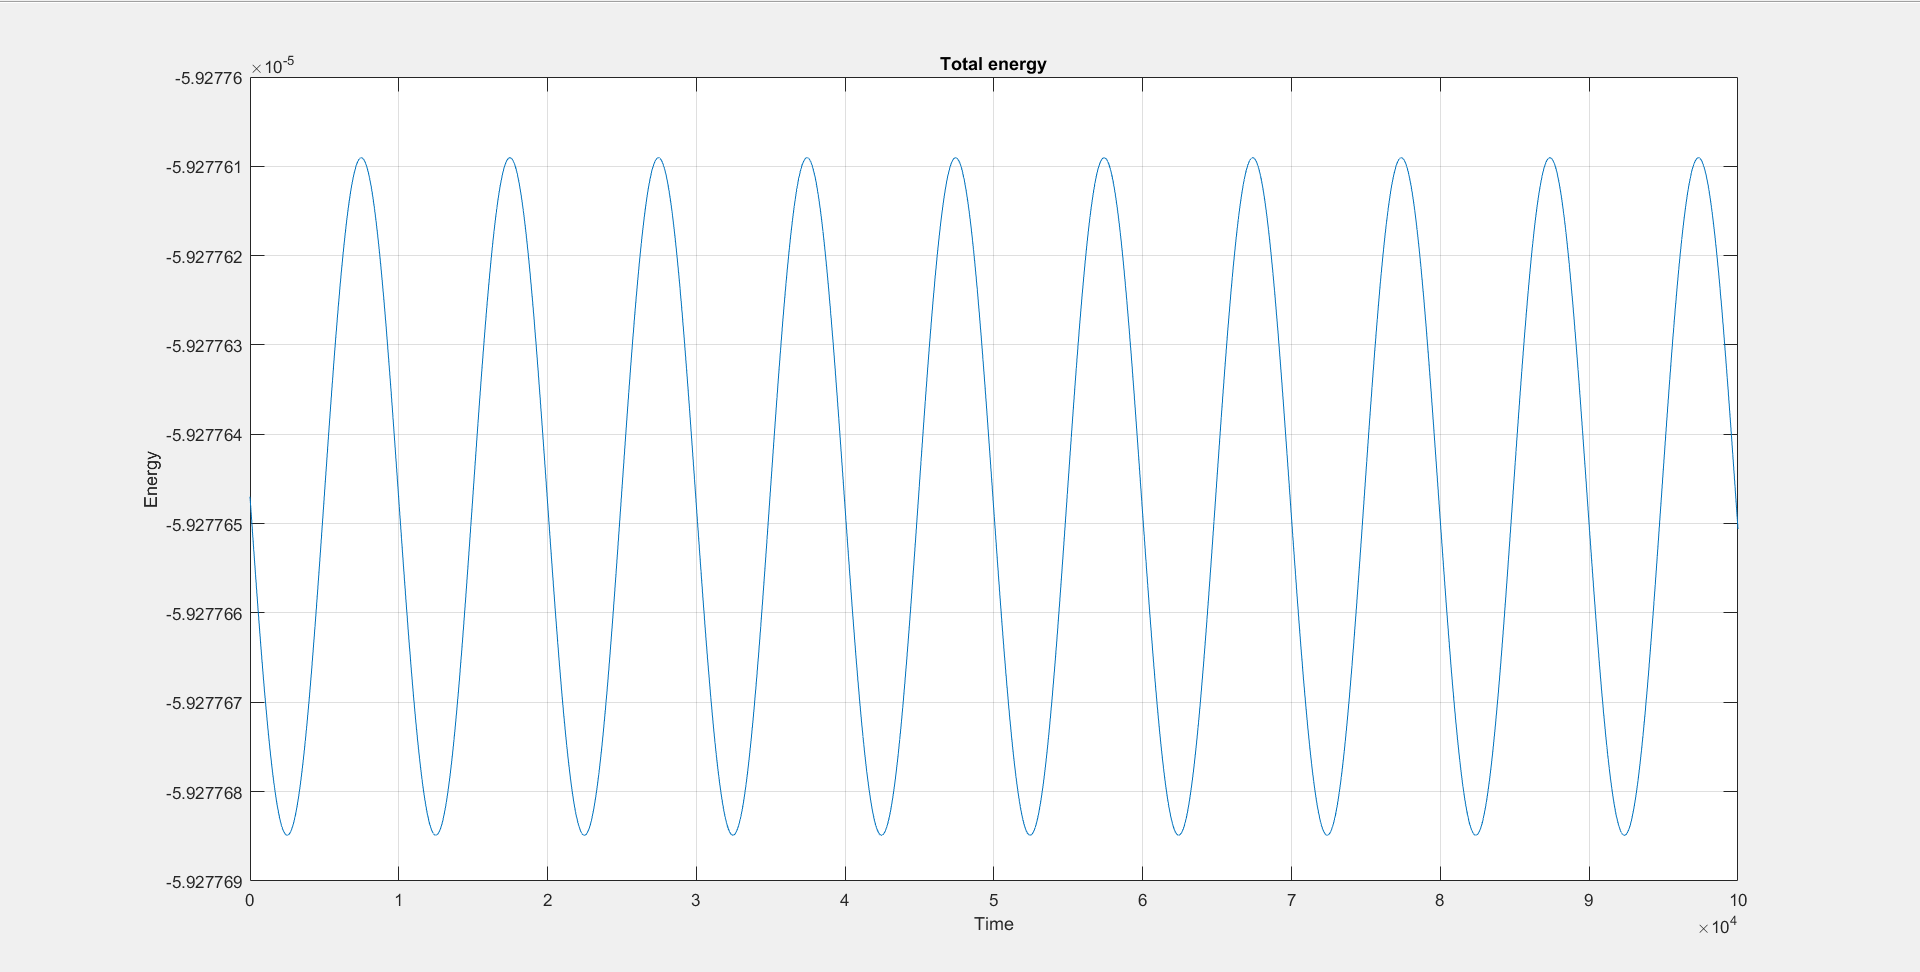
\includegraphics[scale=0.30]{TotalEnergyVerlet.png}}
\caption{The total energy over 10 years, using Eulers forward algorithm. }


\end{figure}

\noindent As there is a circular orbit, the kinetic and potential energies should be conserved, but there will be small small oscillations in energy.\\



\noindent The exact escape velocity of Earth was found to be $v=2\sqrt{2}\pi=8.8857$. By trial and error, the escape velocity was found to be $\approx 8.8$, which is pretty close to the actual velocity. By replacing the gravitational force from

$$
F_G=\frac{GM_{\odot}M_{\mathrm{Earth}}}{r^2}
$$

to

$$
F_G=\frac{GM_{\odot}M_{\mathrm{Earth}}}{r^{\beta}}
$$

\noindent and letting $\beta\in(2,3)$. The orbit becomes increasingly unstable.\\

\begin{figure} [H]  

\centerline{\includegraphics[scale=0.25]{ThreeBody3.jpg}}
\centerline{\includegraphics[scale=0.23]{ThreeBody12.jpg}}
\centerline{ \includegraphics[scale=0.23]{ThreeBody1001.jpg}}
\caption{The planetary orbits of Earth and Jupiter around the sun, with no other interfering forces. Calculated over 50 years with 10000 integration per year. In the last picture the sun is not fixed as center.}
\end{figure}
\noindent The orbit of Earth is affected by the gravitational force of Jupiter. The change is slight for the the case with normal mass. When multiplying Jupiters mass by ten, earth still manages to stay in a slightly shifted orbit. When the mass is multiplied by 1000, earths orbit gets unstable. This is to be expected, as $M_{jup}*1000\approx0.95M_{\odot}$. The sun is not fixed at the center in the last picture, as we wanted to see the development of the free system (figure 3). 


\begin{figure} [H]  
\centerline{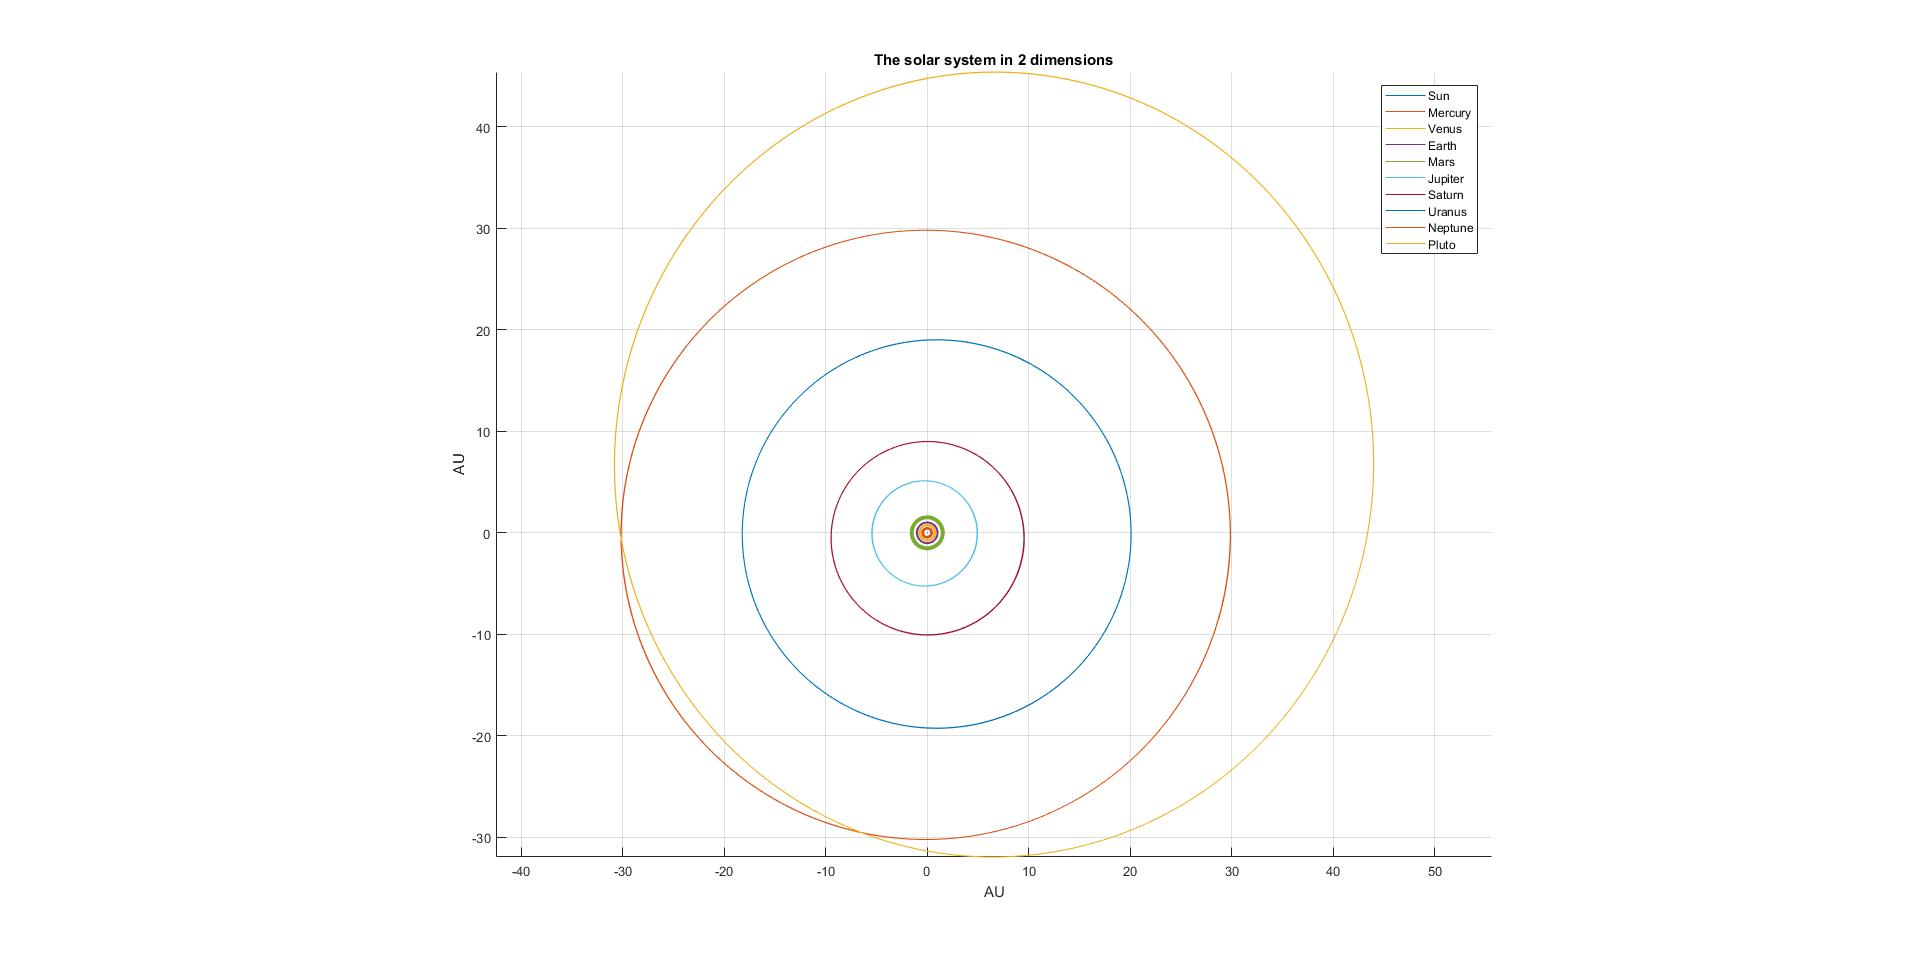
\includegraphics[scale=0.40]{2dsolsys.jpg}}
\caption{The planetary orbits represented in two dimensions for with $10^5$ integration steps over 500 years.}
\end{figure}



\begin{figure} [H]

\centerline{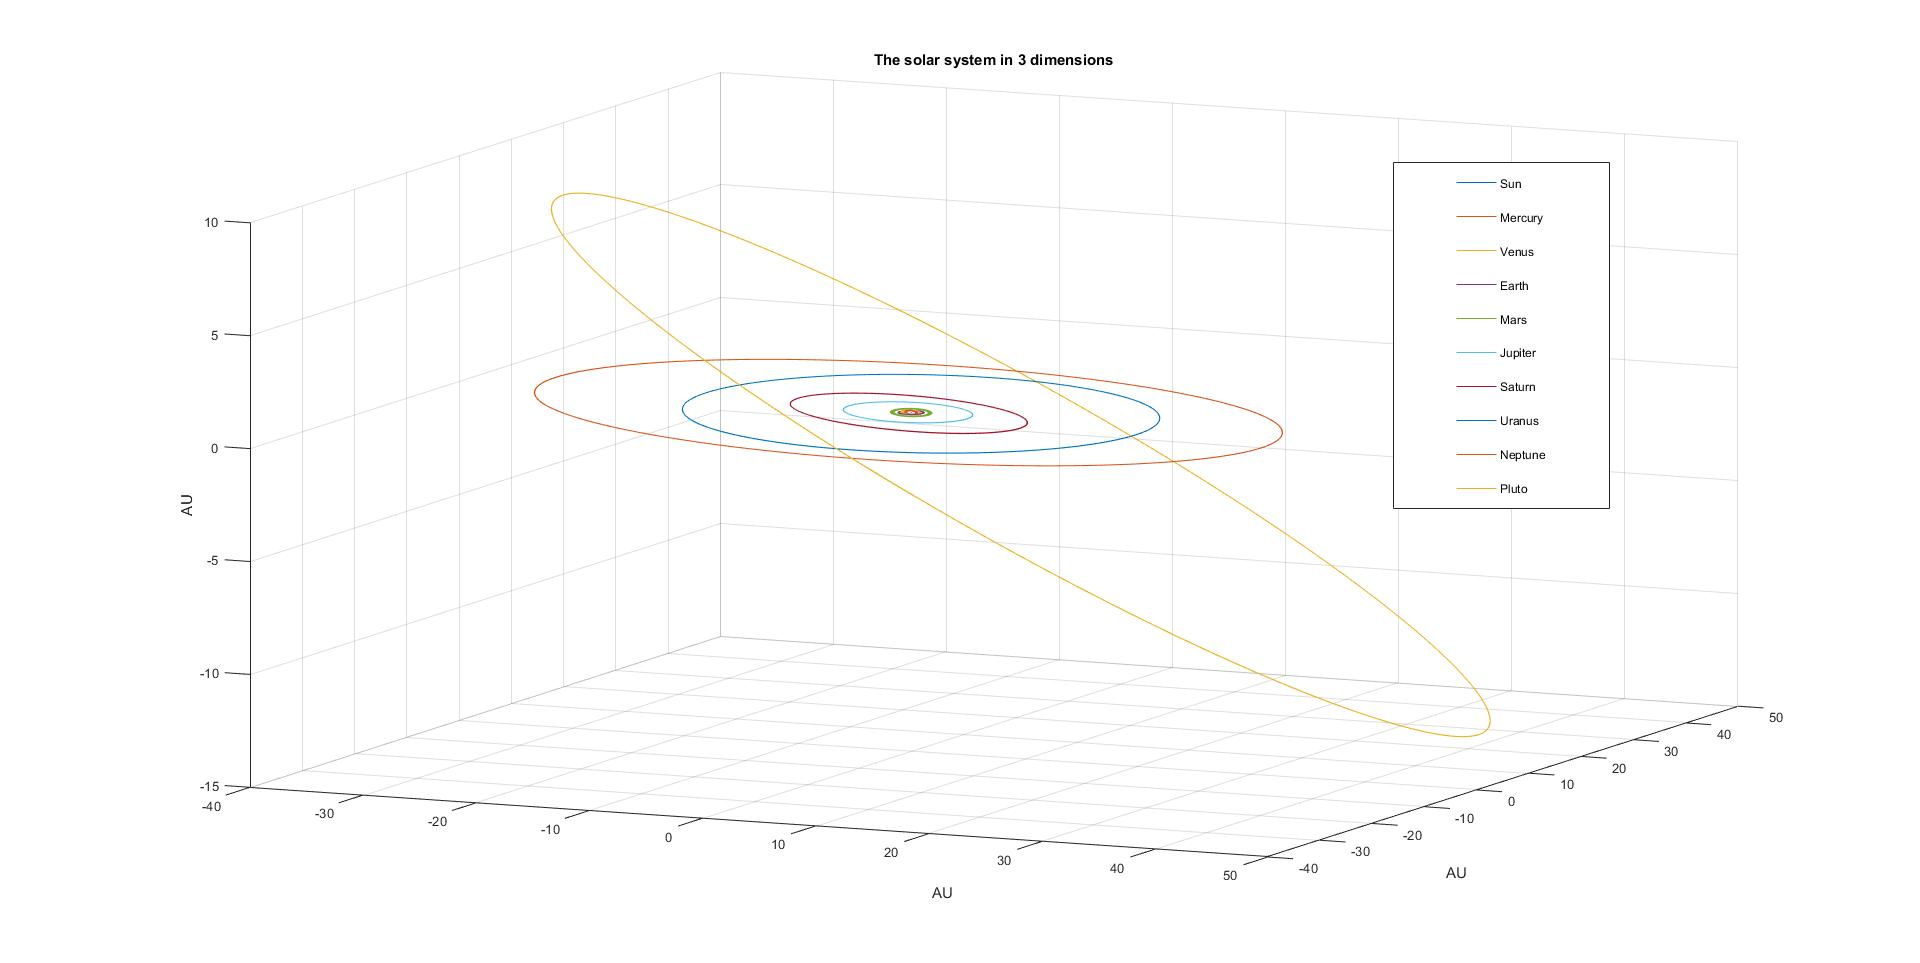
\includegraphics[scale=0.35]{3dsolsys.jpg}}
\caption{The planetary orbits represented in three dimensions for with $10^5$ integration steps over $500$ years.}

\end{figure}

<<<<<<< HEAD
In figure x and y, the solar system is depicted in both 2d and 3d. Almost all the planetary orbits are have stable orbits in the x-y plane. The biggest exception is Pluto (figure y). 
=======
In figure x and y, the solar system is depicted in both 2d and 3d. Almost all the planetary orbits are have stable orbits in the x-y plane. The biggest exception is Pluto (figure y).

>>>>>>> 218c715cc637d816f1e336e4e2e4249c1ebfb8c6

\begin{figure}
\centerline{\includegraphics[scale=0.4]{perihelion100mill.jpg}}
\caption{The perihelion precession of Mercury computed over one century with 100 million integration points}
\end{figure} 

\newpage
{\LARGE\bf
Discussion
}
\\
<<<<<<< HEAD
Stability of algorithms:\\


\noindent The Euler forward method is easy for the computer to handle, but it is not robust for few integration points. The number of FLOPS in the Euler forward algorithm is 5n-flops. Compared to the velocity verlet algorithm, that uses 9n flops, the Euler algorithm is faster. The velocity verlet gets more out of each rotation, hence is more robust for fewer integration points. The potential and kinetic energy oscillates, but is generally conserved over one orbit(figure noe). This is because of the circular orbit,  \\

\noindent The escape velocity of Earth is exactly $v_e=2\sqrt{2}\pi$. This corresponded quite well with the velocity found by trial and error. When the gravitational force was changed by replacing $r^2\rightarrow r^\beta$, the orbit got unstable. The gravitational force will be stronger for low $r$, resulting in higher velocities. The force will decrease more rapidly at higher $r$. This can work like a slingshot-effect, making stable orbits harder to obtain.  

=======



\noindent The Euler forward method is easy for the computer to handle, but it is not robust for few integration points. The number of FLOPS in the Euler forward algorithm is 5n-flops. Compared to the velocity verlet algorithm, that uses 9n flops, the Euler algorithm is faster. This is shown in table 1. The velocity verlet gets more out of each rotation, hence is more robust for fewer integration points. The velocity that makes a circular orbit is $v=2\pi$. This is pretty logical given the choice of units. As the radius of Earths orbit per definition is 1 AU and the circumference is given by $2\pi r$, the velocity of Earth has to be $2\pi \frac{AU}{year}$ in order to do a full rotation per year. The potential and kinetic energy oscillates, but is generally conserved over one orbit(figure 2). The angular momentum is also conserved. These quantities should be conserved if a planet is an idealized circular orbit, as the radius and velocity is constant.  \\

\noindent The escape velocity of Earth is exactly $v_e=2\sqrt{2}\pi$. This corresponded quite well with the velocity found by trial and error. When the gravitational force was changed by replacing $r^2\rightarrow r^\beta$, where $\beta \in(2,3)$, the orbit got unstable. The gravitational force will be stronger for low $r$, resulting in higher velocities. The force will decrease more rapidly at higher $r$. This can work like a slingshot-effect, making stable orbits harder to obtain.  
>>>>>>> 218c715cc637d816f1e336e4e2e4249c1ebfb8c6






\newpage
{\LARGE\bf
Conclusion
}









\newpage
{\LARGE\bf
References
}











\end{document}